% Syslab Research Journal Template
% By Patrick White
% September 2019

% Do not edit this header
\documentclass[letterpaper,11pt]{article}
\usepackage{fullpage}
\usepackage{palatino}
\usepackage{enumitem}
\usepackage{courier}
\usepackage{graphicx}
\def\hrulefill{\leavevmode\leaders\hrule height 20pt\hfill\kern\z@}

% ------------- Edit these definitions ---------------------
\def\name{Bryan Lu}
\def\journalnum{12}
\def\daterange{12/9/19-12/16/19} % starts on Monday
\def\period{2}
% ------------------ END ---------------------------------
% Do not edit this
\begin{document}
	\thispagestyle{empty}
	\begin{flushright}
		{\Large Journal Report \journalnum} \\
		\daterange\\
		\name \\
		Computer Systems Research Lab \\
		Period \period, White
		\end{flushright}
	\hrule height 1pt

% ------ SECTION DAILY LOG -------------------------------------
\vspace{-0.8em}
\section*{Daily Log}
%Detail for each day about what you research, coded, debug, designed, created, etc. Informal style is OK.
\vspace{-0.8em}
\subsection*{Monday, December 9}
\vspace{-0.6em}
Downloaded testcases from the project website and looked into how the testcases are accessed by the code from the \texttt{database} directory. 
\vspace{-1.3em}
\subsection*{Tuesday, December 10}
\vspace{-0.6em}
Picked apart the main method in the \texttt{text} subdirectory of the original code that does the training and learning, and understood what the main method accepts and outputs. 
\vspace{-1.3em}
\subsection*{Thursday, December 12}
\vspace{-0.6em}
Began modifying the \texttt{ontology} and \texttt{database} subdirectories and figured out what files to modify in order to accommodate my additional methods. 
\vspace{-0.8em}

% ------ SECTION TIMELINE -------------------------------------
%\newpage
%\vspace{-1.7em}
\vspace{-1.0em}
\section*{Timeline}
\begin{tabular}{|p{1in}|p{2.5in}|p{2.5in}|}
	\hline
\textbf{Date} & \textbf{Goal} & \textbf{Met}\\ \hline 
	\hline
11/25 & Build, test, and train the logistic model, given the test data and the features computed. & No, Thanksgiving break -- did not do work on the project over break. \\
	\hline 
12/2 & Refine logistic learning model with extra methods to try to increase accuracy, and begin extracting the most likely literals. & Unclear how to do this from my work so far, found a different approach to continue work. \\
	\hline 
12/9 & Inject my problem statements, lexicon, and files into the existing framework given by the original project. & I've begun this process, but it's taken a while to figure out what each file and component does. \\
	\hline 
12/16 & Harness the existing code and overhaul the \texttt{ontology} directory and test case code to fit my project. & N/A \\
	\hline 
12/23 & Over break, run part of the code successfully to output a set of literals naively constructed from the problem statement.  & N/A \\ 
	\hline 
Winter Goal & Be able to output a set of possible literals (statements) based on detected relations in the problem. & N/A \\
	\hline 
\end{tabular}

\pagebreak 
% ------ SECTION REFLECTION  ---------------------------------
\section*{Reflection}
%In narrative style, talk about your work this week. Successes, failures, changes to timeline, goals. This should also include concrete data, e.g. snippets of code, screenshots, output, analysis, graphs, etc.

Over the past week, I've spent most of my time poring over the Github code and understanding how all of the pieces mentioned in the original paper fit together. Generally, with regards to the text-parsing side of their original problem, they access the problems and annotations for those problems from a local database and run them through one of Stanford's Natural Language Processing libraries to get all sorts of features and data from each statement. These sentence features (what the paper calls ``syntax parses'') are then fed into a Naive Tag Model, along with the ``annotations'' for each test case. 

Here is the basic directory of all the relevant code to the paper's overall project: 
\begin{center}
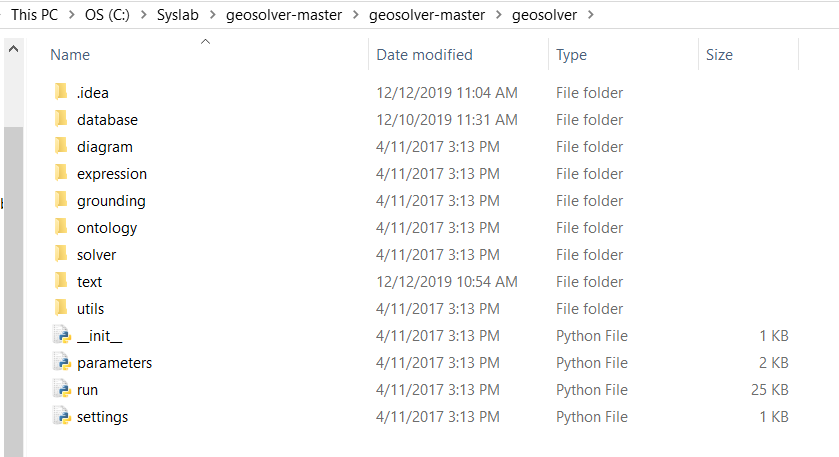
\includegraphics[width=0.5\textwidth]{directory.png}\\
\end{center}
The \texttt{diagram} and \texttt{solver} directories are useless for my purposes -- those were intended to be used to parse pictures of SAT geometry problems and to solve them explicitly based on answer choices, which aren't tasks my project is looking into. The \texttt{database} directory gives code for uploading/downloading test cases and questions, which I don't find wholly necessary, but I will likely use it at some point. The \texttt{ontology} directory contains information about the logical language the project is already using (with the \texttt{pyparser} package), and there are obvious places to add the items in my \texttt{lexicon.txt} to make it complete. Appropriately, the \texttt{text} directory contains all of the code for text-parsing, and I find that the main method in that directory is likely what I will be running as a part of my final project. 

The greatest thing about finding this code is that the amount of building that I have to do myself has been essentially axed -- I just have to repurpose/refurbish it. It's currently written in Python 2, so I have to update the syntax a little, and I have to modify the input/output, but that's not as daunting as a task as before. I'm just not sure yet how my test cases for training fit in with the rest of the model yet. Hence, the first thing I will do Monday morning is to send the authors of the paper an email asking about how to do this task, and hopefully I can get very close to my winter goal by the end of this week. I'm not sure if completing it is as reasonable as I once thought, however, but it's certainly more achievable than before. 

\end{document}

